\begin{figure*}[t]
\centering
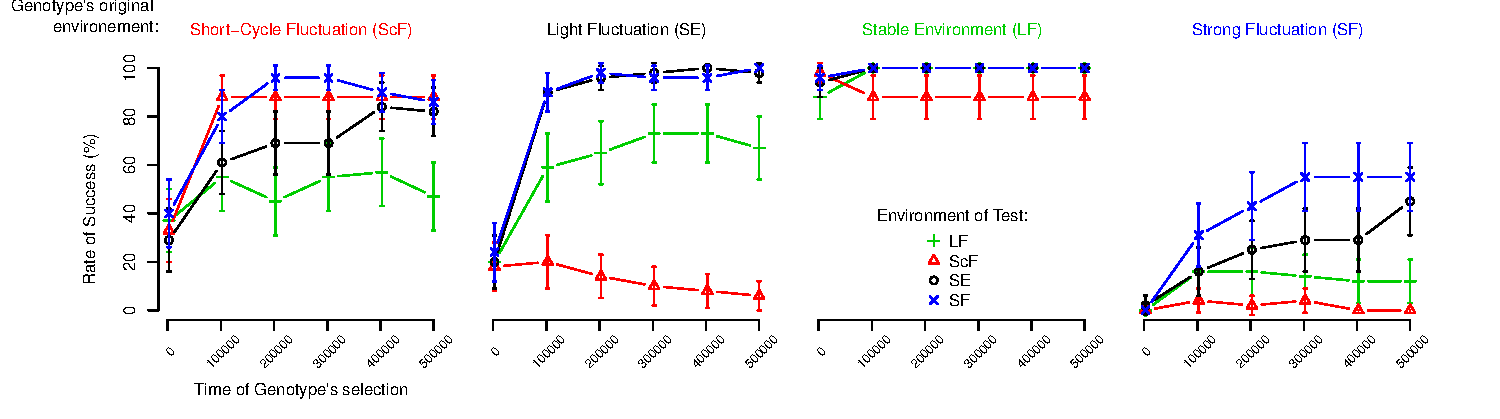
\includegraphics[width=2\columnwidth]{img/testSurvivingRates}
\caption{Success rate of genotypes in homogeneous tests.}
\label{fig:survrate}
\end{figure*}

\subsection{Environmental Transitions}

Figure~\ref{fig:trans} visualizes the average transition between environments in different homogeneous runs. To compute this typical transition we averaged the phenotypic disturbance $P$ over iterations $[t-40, t+40]$ for all $t \ge 5,000$ and $t \in T_r$, where $T_r$ is the sequence of iterations of run $r$ at which a transition between environments effectively occurred, i.e. for which $E(t) \ne E(t+1)$. Figure~\ref{fig:transonly} shows the average transitions of ScF genotypes collected at the 6 aforementioned time steps \{2,500, 102,500, ..., 500,000\} and subjected to a homogeneous ScF test. It shows that phenotypes of the genotypes collected later in the evolutionary process are less sensitive to environmental fluctuations. Conversely, as reported in Figure~\ref{fig:transli}, the phenotypes of genotypes from SF keep the same high sensitivity regardless of the iteration at which they were collected. Finally, figures~\ref{fig:transst} and~\ref{fig:transstest} compare the average transitions in homogeneous ScF and SF tests with genotypes collected at iteration 500,000 from the four different configurations. Again, it can be observed here that the phenotype of ScF is much more stable than the others in its original environment. On the contrary, it is very sensitive to transitions in SF. High sensitivity to fluctuations includes both individuals which developed plasticity and those which fail to resist the environmental fluctuations.

\subsection{Phenotypic Diversity} 

The phenotypic diversity measured in Figure~\ref{fig:phenodiv} can also be observed relatively easily by visual inspection of the CA as displayed in the few screenshots of Figure~\ref{fig:phenoexpl}. First, LF and SF are visibly different from ScF. These two groups diverge substantially in texture and also clearly differ from SE. Individuals from ScF seem to produce stable and robust phenotypes in any environment encountered within a ScF scheme. Their adaptations appear essentially created by genotypic mutations and their plasticity is low. They are also very dependent on their original ecosystem, sometimes distinctively as depicted in Figure~\ref{fig:smalldistinctive}, and consequently not robust in other types of fluctuations, where the effect of mutations is probably enhanced by the reduced size of the genotypes as mentioned previously. By contrast, individuals evolved within LF or SF appear to possess great plasticity, their phenotypic diversity is high, and it seems likely that phenotypic selection occurs despite the fact that their genotypic diversity is lower.

\begin{figure}[h]
\begin{subfigure}{.25\textwidth}
 \centering
 \includegraphics[width=.7\linewidth, angle =-90]{img/boxendingsFailedstable.eps}
 \caption{SE}
 \label{fig:sfig1}
\end{subfigure}%
\begin{subfigure}{.25\textwidth}
 \centering
 \includegraphics[width=.7\linewidth, angle =-90]{img/boxendingsFailedvariation.eps}
 \caption{SF}
 \label{fig:sfig2}
\end{subfigure}
\begin{subfigure}{.25\textwidth}
 \centering
 \includegraphics[width=.7\linewidth, angle =-90]{img/boxendingsFailedvariationLight.eps}
 \caption{LF}
 \label{fig:sfig2}
\end{subfigure}%
\begin{subfigure}{.25\textwidth}
 \centering
 \includegraphics[width=.7\linewidth, angle =-90]{img/boxendingsFailedvariationSmall.eps}
 \caption{ScF}
 \label{fig:sfig1}
\end{subfigure}
\caption{Last iterations reached by living cells of homogeneous runs that died out before 60,000 iterations.}
\label{fig:ending}
\end{figure}

\begin{figure}[h]
\begin{subfigure}{.25\textwidth}
 \centering
 \includegraphics[width=.7\linewidth, angle =-90]{img/Sucavg499999variationb.eps}
 \caption{SF: genomes from $t\!=\!50,000$.}
 \label{fig:transst}
\end{subfigure}%
\begin{subfigure}{.25\textwidth}
 \centering
 \includegraphics[width=.7\linewidth, angle =-90]{img/SucavgvarValidvariationb.eps}
 \caption{SF: genomes from SF.}
 \label{fig:transli}
\end{subfigure}
\begin{subfigure}{.25\textwidth}
 \centering
 \includegraphics[width=.7\linewidth, angle =-90]{img/Sucavg499999variationSmallb.eps}
 \caption{ScF: genomes from $t\!=\!50,000$.}
 \label{fig:transstest}
\end{subfigure}%
\begin{subfigure}{.25\textwidth}
 \centering
 \includegraphics[width=.7\linewidth, angle =-90]{img/SucavgvarSmallValidvariationSmallb.eps}
 \caption{ScF: genomes from ScF.}
 \label{fig:transonly}
\end{subfigure}
\caption{Phenotypic disturbance: Average transition between environments in different types of homogeneous tests.}
\label{fig:trans}
\end{figure}

\begin{figure}
\begin{subfigure}{.25\textwidth}
 \centering
 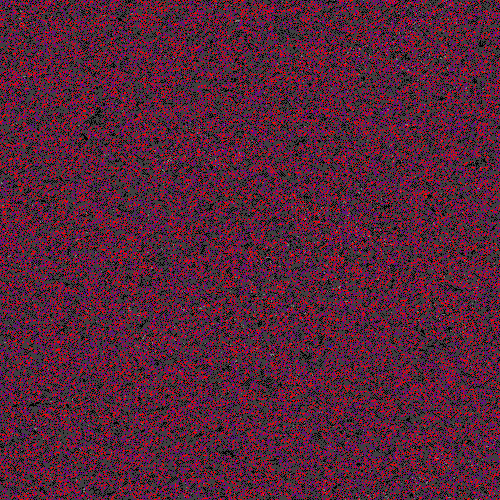
\includegraphics[width=.9\linewidth]{img/stable495000}
 \caption{SE}
\end{subfigure}%
\begin{subfigure}{.25\textwidth}
 \centering
 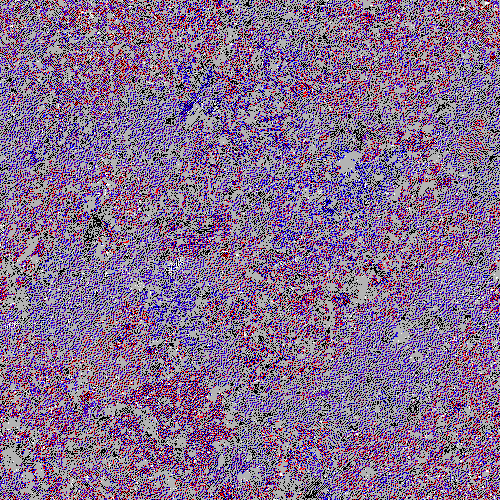
\includegraphics[width=.9\linewidth]{img/var495000}
 \caption{SF}
\end{subfigure}
\begin{subfigure}{.25\textwidth}
 \centering
 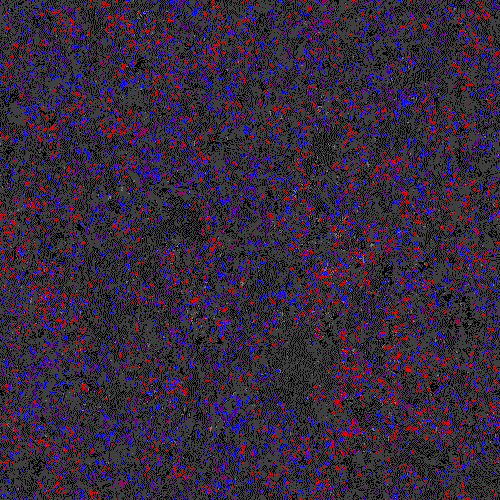
\includegraphics[width=.9\linewidth]{img/light495000}
 \caption{LF}
\end{subfigure}%
\begin{subfigure}{.25\textwidth}
 \centering
 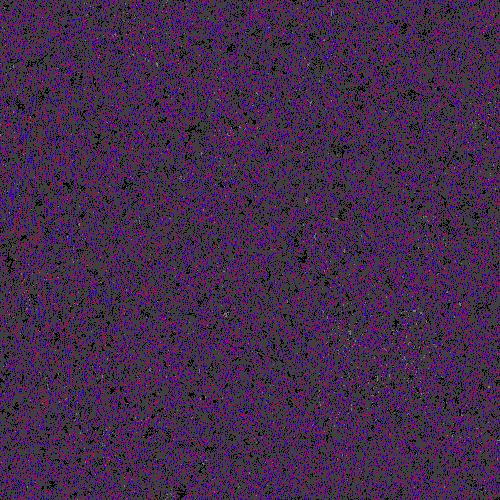
\includegraphics[width=.9\linewidth]{img/small495000}
 \caption{ScF}
\end{subfigure}
\caption{Screenshots of the CA. Grid state distribution (phenotype) at iteration 495,000 for the four different configurations. Each cell state is represented by a different color. Black and grey represent cells in the \emph{decay} and \emph{quiescent} states, respectively. Shades of blue, red and purple represent the living states.}
\label{fig:phenoexpl}
\end{figure}

\begin{figure}
\begin{subfigure}{.12\textwidth}
 \centering
 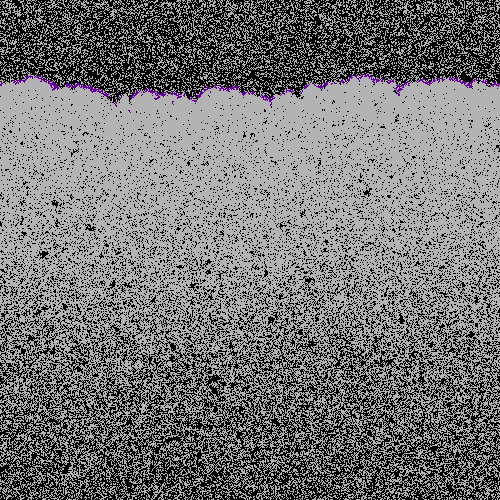
\includegraphics[width=1\linewidth]{img/sm100000}
 \caption{$t=100,000$}
\end{subfigure}%
\begin{subfigure}{.12\textwidth}
 \centering
 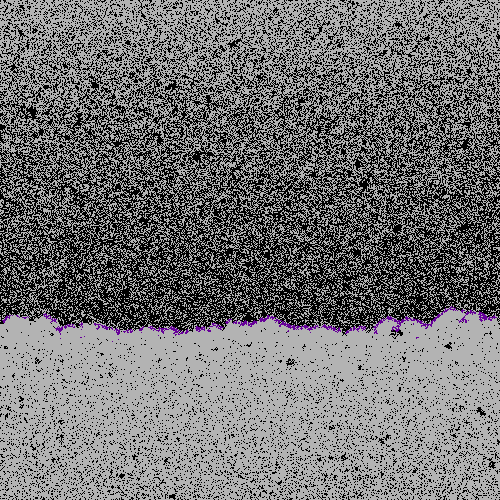
\includegraphics[width=1\linewidth]{img/sm200000}
 \caption{$t=200,000$}
\end{subfigure}%
\begin{subfigure}{.12\textwidth}
 \centering
 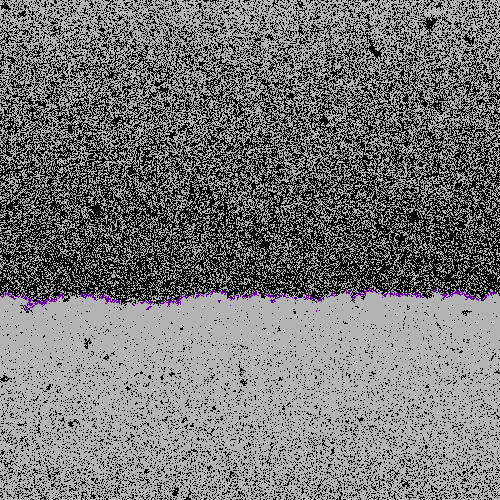
\includegraphics[width=1\linewidth]{img/sm400000}
 \caption{$t=400,000$}
\end{subfigure}%
\begin{subfigure}{.12\textwidth}
 \centering
 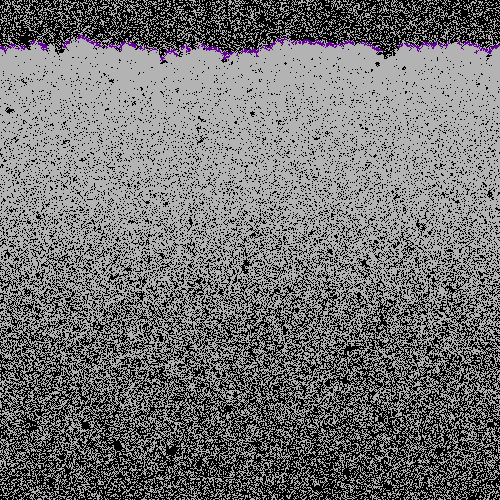
\includegraphics[width=1\linewidth]{img/sm500000}
 \caption{$t=500,000$}
\end{subfigure}
\caption{Original ScF simulation: a distinctive ``wavy'' phenotype, very stable over time, produces genotypes that fail in the early iterations of the homogeneous test.}
\label{fig:smalldistinctive}
\end{figure}
